

\documentclass[a4paper, 12pt]{article} 
\usepackage{amsmath, amssymb, color, graphicx, enumitem}
\usepackage{fullpage} %smaller margins
\usepackage{hyperref} % hyperlinks
\usepackage{mdframed} %for boxes

%font
%\usepackage[sc]{mathpazo}
%\linespread{1.05}         % Palladio needs more leading (space between lines)
%\usepackage[T1]{fontenc}

%font, libertine
\usepackage{libertine}

%word spacing
\usepackage{microtype}

%all equations get full space
\everymath{\displaystyle}

%useful shortcuts
\def\R{\ensuremath{\mathbb{R}}} %\ensuremath adds math mode, if forgotten
\def\Q{\ensuremath{\mathbb{Q}}}
\def\N{\ensuremath{\mathbb{N}}}
\def\Z{\ensuremath{\mathbb{Z}}}
\def\C{\ensuremath{\mathbb{C}}}

%shorcuts with arguments
\newcommand{\abs}[1]{\left\vert#1\right\vert} %nice absolute values
\newcommand{\bt}[1]{\textbf{#1}} %bold
\newcommand{\eq}[1]{\begin{align*}#1\end{align*}} %aligned equations
\newcommand{\norm}[1]{\left\lVert#1\right\rVert} %vector norm
\newcommand{\notimplies}{% does not imply
  \mathrel{{\ooalign{\hidewidth$\not\phantom{=}$\hidewidth\cr$\implies$}}}}
\renewcommand{\eq}[1]{\begin{align*}#1\end{align*}} %aligned equations

%piecewise function

%\begin{displaymath}
%   f(x) = \left\{
%     \begin{array}{lr}
%       1 & : x \in \mathbb{Q}\\
%       0 & : x \notin \mathbb{Q}
%     \end{array}
%   \right.
%\end{displaymath} 

%colors
\definecolor{javagreen}{rgb}{0.25,0.5,0.35} %dark green color
\definecolor{lightblue}{rgb}{0.149,0.545,0.824} %solarized blue
\definecolor{sred}{rgb}{0.863, 0.196, 0.184} %solarized red

\newcommand{\blue}[1]{{\leavevmode\color{lightblue}{#1}}} %solarized blue 
\newcommand{\green}[1]{{\leavevmode\color{javagreen}{#1}}} %command for green
\newcommand{\red}[1]{{\leavevmode\color{sred}{#1}}} %solarized red
\newcommand{\gray}[1]{{\leavevmode\color[gray]{0.5}{#1}}} %gray text

%environment
\newcommand{\tab}{\phantom{ssss}}

\title{}
\date{}
%==tips====
%part
    %section, sub, sub
%\begin{enumerate}[resume] %continues counting
\begin{document}
\begin{center}
\section*{Traversal Algorithm}
\end{center}

\begin{tabular}{ c  c c } 
\bt{article} & & \bt{first link } \\
 A & $\rightarrow$&  B\\ 
 B & $\rightarrow$&  C\\ 
 C & $\rightarrow$&  A\\ 
 D & $\rightarrow$&  C\\ 
 E & $\rightarrow$&  C\\ 
 F & $\rightarrow$&  E\\ 
 G & $\rightarrow$&  E\\ 
\end{tabular}

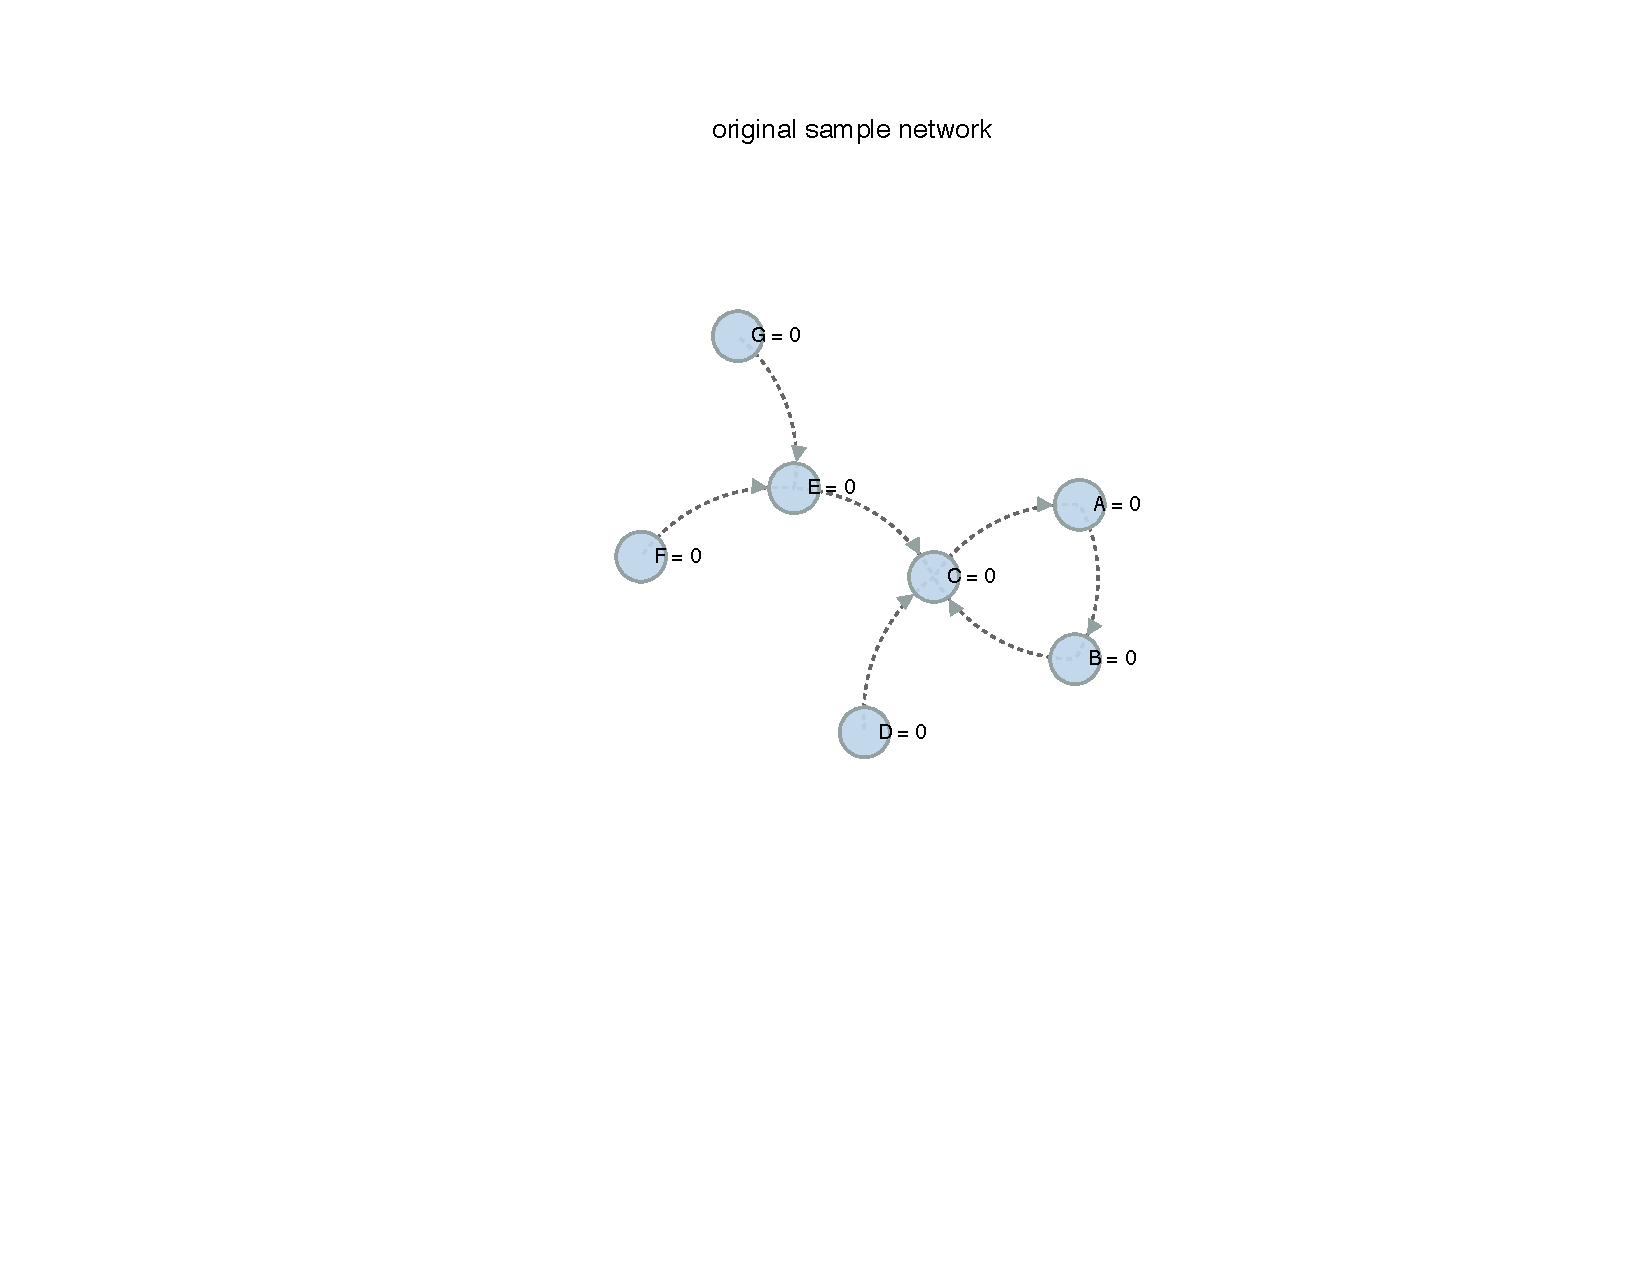
\includegraphics[width=\textwidth]{traversal_algo_org_net.pdf}    
\newpage
{\large \bt{Traversal Visit Matrix}\\


$\begin{bmatrix}
    \vec A_{\text{visit}}   \\
    \vec B_{\text{visit}}   \\
    \vec C_{\text{visit}}   \\
   \vec D_{\text{visit}}   \\
    \vec E_{\text{visit}}   \\
    \vec F_{\text{visit}}   \\
    \vec G_{\text{visit}}   \\
\end{bmatrix}
=
\begin{bmatrix}
    1 & 1 & 1 & 1 & 1 & 1 & 1  \\
    1 & 1 & 1 & 1 & 1 & 1 & 1  \\
    1 & 1 & 1 & 1 & 1 & 1 & 1  \\
    0 & 0 & 0 & 0 & 0 & 0 & 0 \\
    0 & 0 & 0 & 0 & 0 & 1 & 1 \\ %E
    0 & 0 & 0 & 0 & 0 & 0 & 0 \\
    0 & 0 & 0 & 0 & 0 & 0 & 0 \\
\end{bmatrix}
$

The number of \bt{traversal visits} for article $A =$
$ \sum_{i=1}^{i=7} \vec A_{\text{visit, }i} = 7 $ \\
{\small\ \ \ \gray{(sum of entries in $\vec A_{\text{visit}}$)}} \\

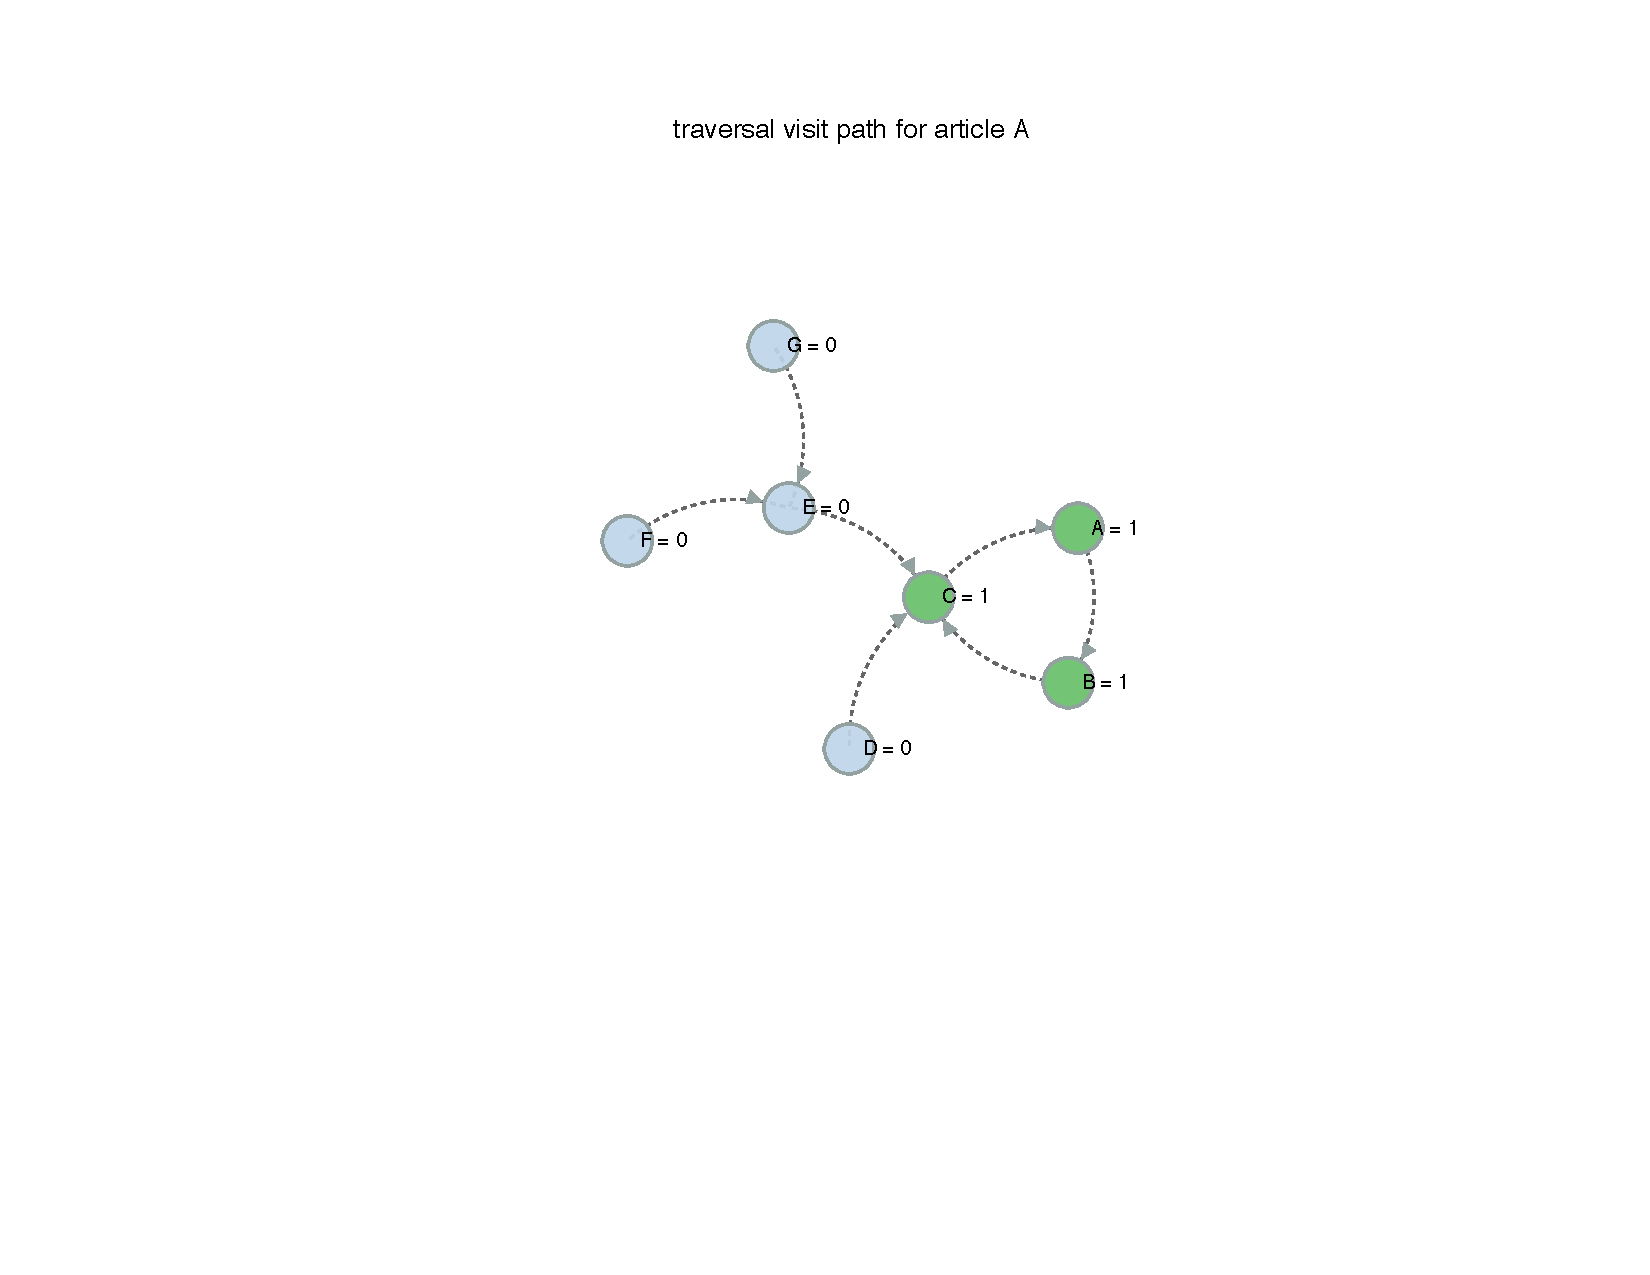
\includegraphics[width=\textwidth]{traversal_algo_A.pdf}    

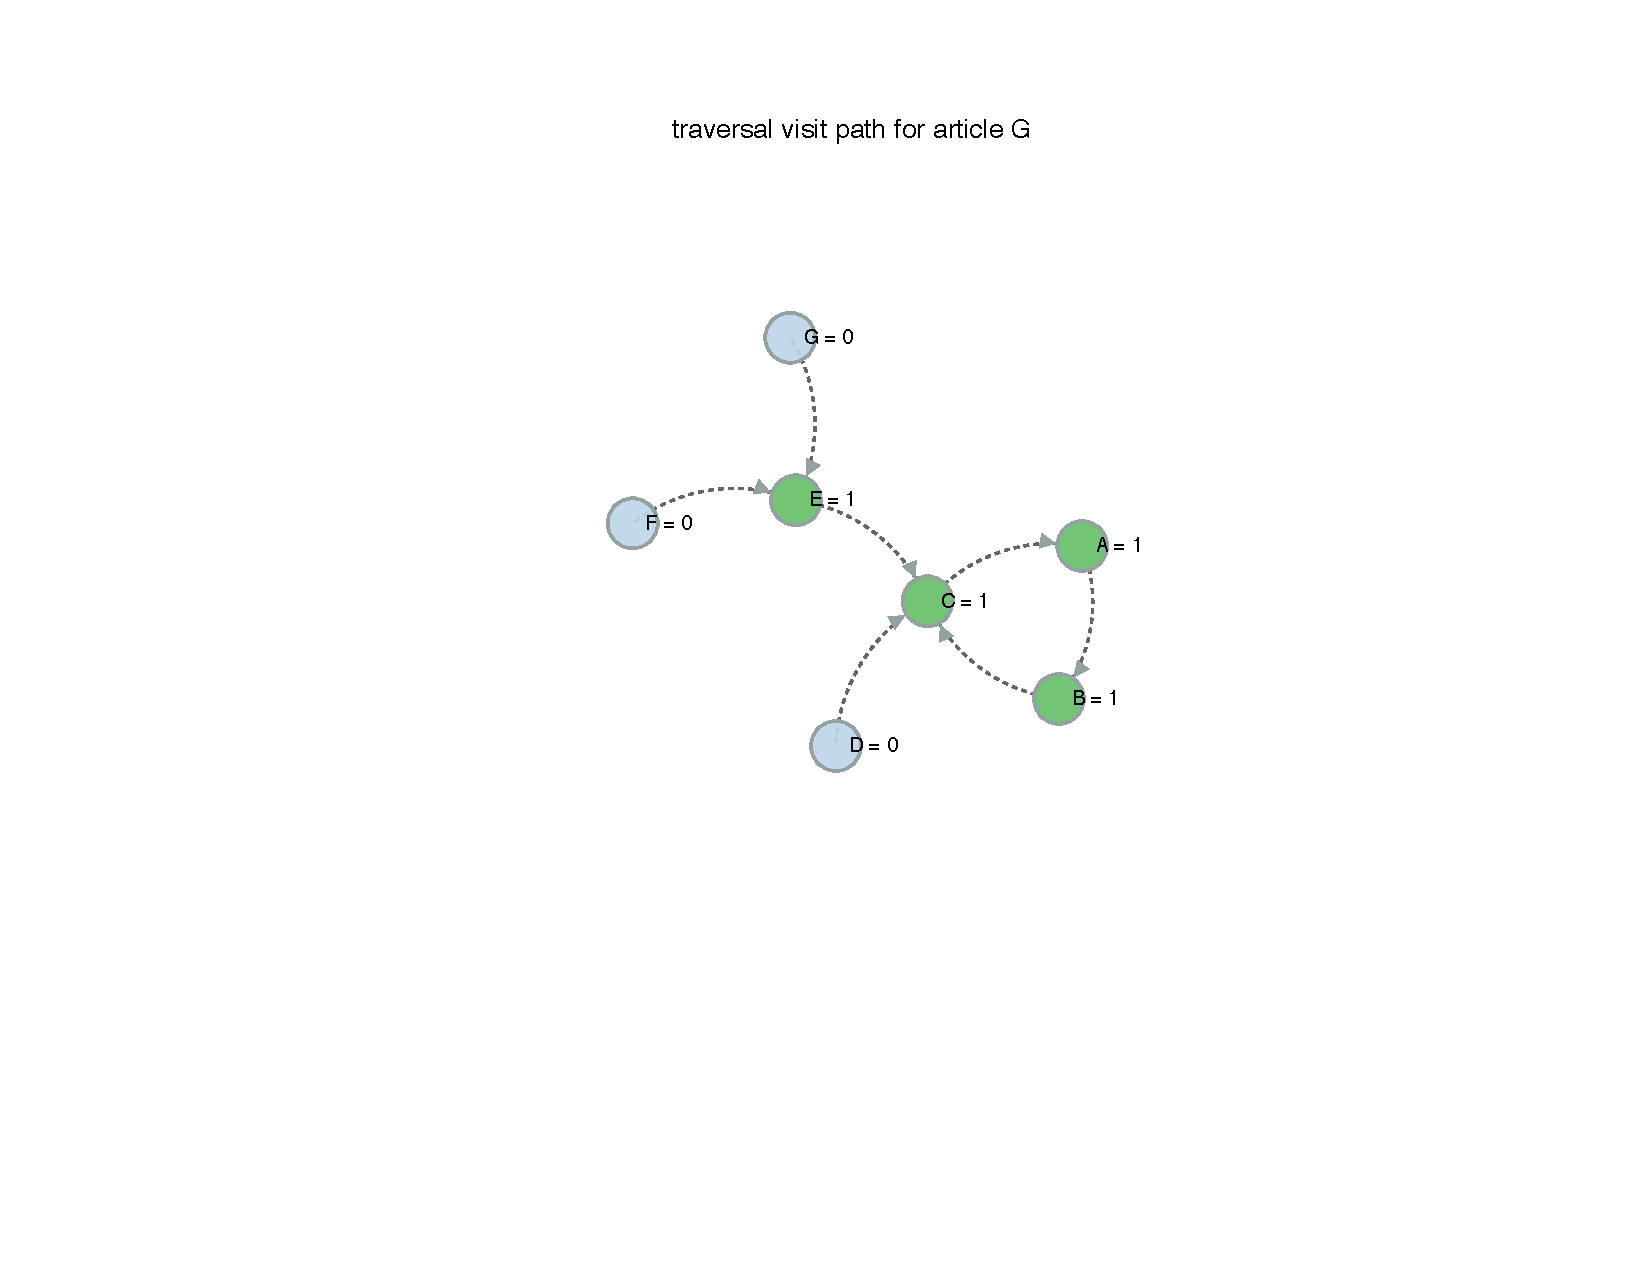
\includegraphics[width=\textwidth]{traversal_algo_G.pdf}    
%insert A path
\vspace{1cm}


{\large \bt{Traversal Funnel Matrix}}\\


$\begin{bmatrix}
   \vec A_{\text{funnel}}   \\
   \vec    B_{\text{funnel}}   \\
   \vec C_{\text{funnel}}   \\
   \vec D_{\text{funnel}}   \\
   \vec E_{\text{funnel}}   \\
    \vec F_{\text{funnel}}   \\
    \vec G_{\text{funnel}}   \\
\end{bmatrix}
= 
\begin{bmatrix}
    0 & 0 & 0 & 0 & 0 & 0 & 0\\
    0 & 0 & 0 & 0 & 0 & 0 & 0\\
    0 & 0 & 0 & 1 & 1 & 1 & 1\\
    0 & 0 & 0 & 0 & 0 & 0 & 0\\
    0 & 0 & 0 & 0 & 0 & 1 & 1\\ %D
    0 & 0 & 0 & 0 & 0 & 0 & 0\\
    0 & 0 & 0 & 0 & 0 & 0 & 0\\
\end{bmatrix}
$
\vspace{2cm}


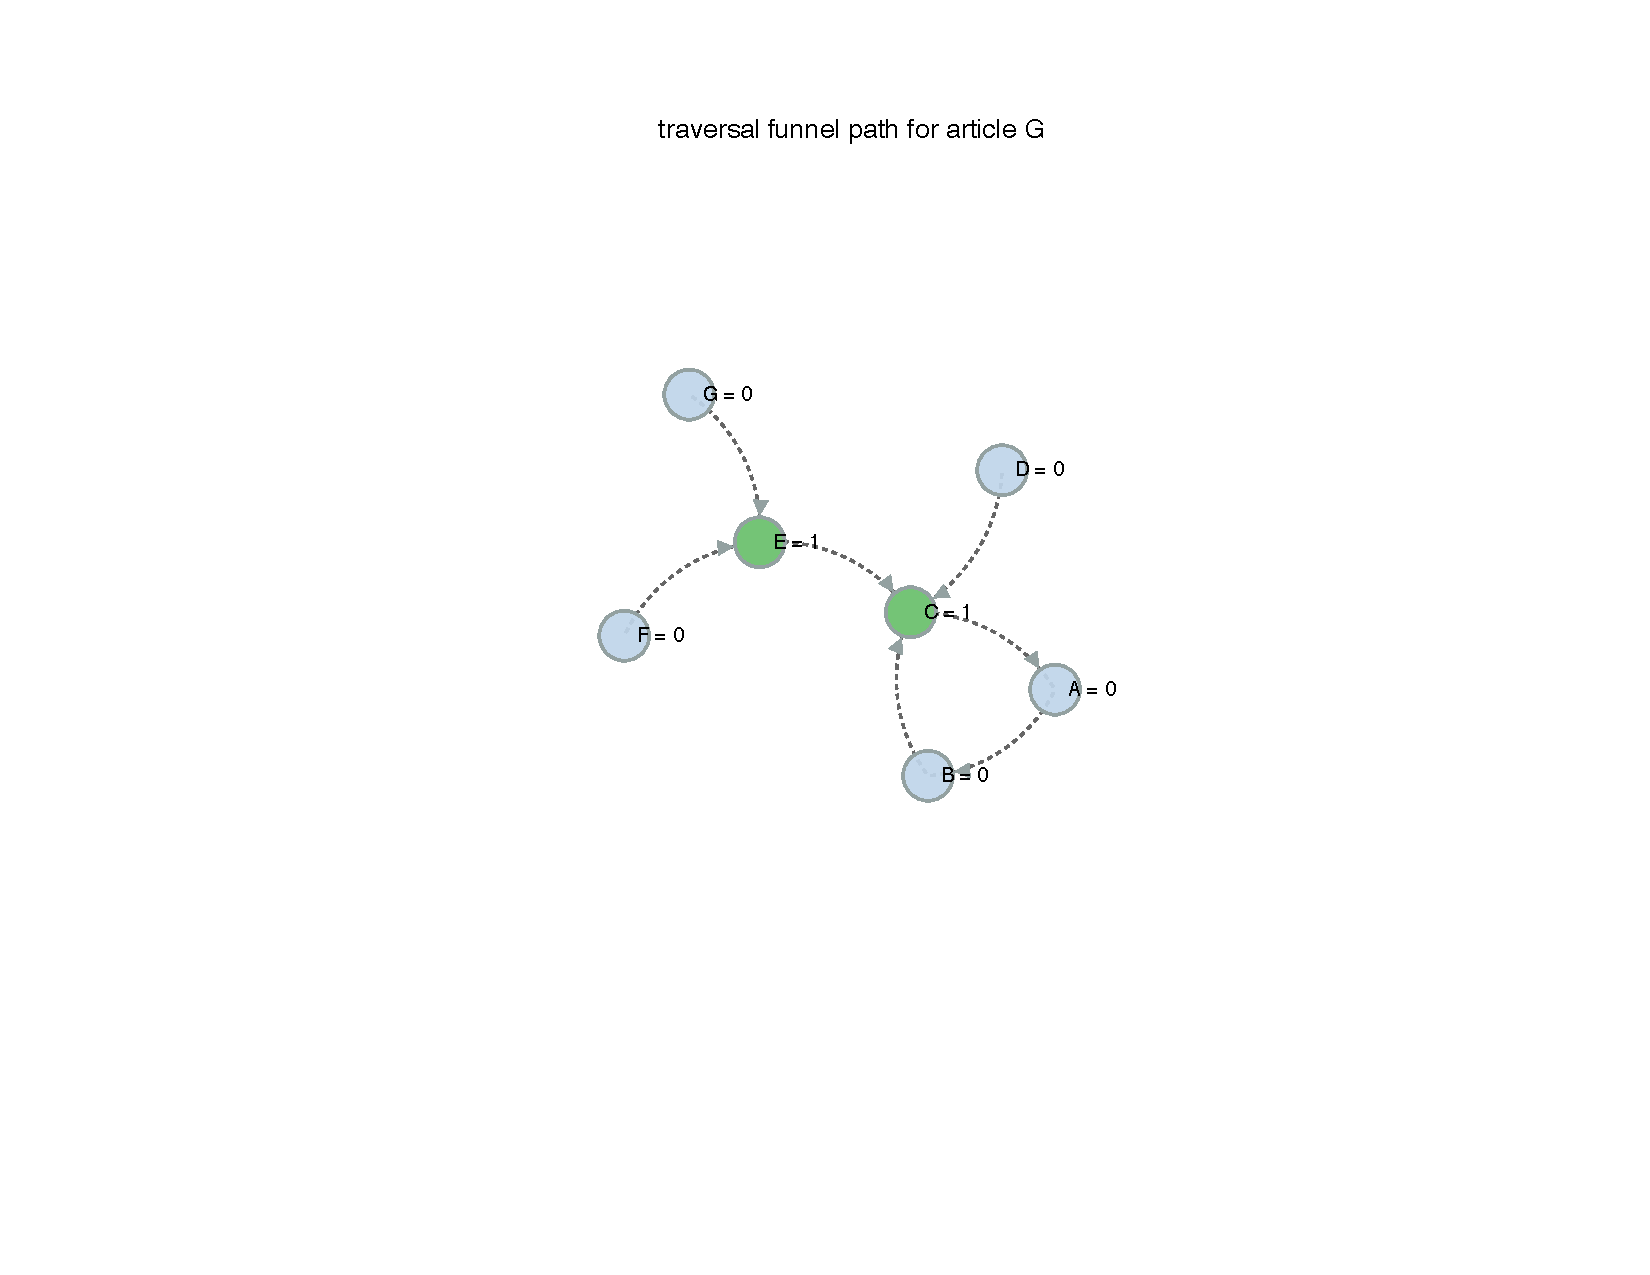
\includegraphics[width=\textwidth]{traversal_funalgo_G.pdf}    



The number of \bt{traversal funnels} for article $E =$
$ \sum_{i=1}^{i=7} \vec E_{\text{funnel, }i} = 2 $ \\
{\small\ \ \ \gray{(sum of entries in $\vec E_{\text{funnel}}$)}} \\

\end{document}

